\begin{frame}
	\frametitle{Modelos em Economia}

	\begin{center}
		{\huge Modelos em Economia}
	\end{center}

\end{frame}

\begin{frame}
	\frametitle{Modelos em Economia}
	\begin{center}
		\includegraphics[scale=0.3]{metro.png}
	\end{center}

\end{frame}

\begin{frame}
	\frametitle{Modelos em Economia}
	\begin{itemize}
		\item S\~ao uma forma de ultrapassar a complexidad da realidad e evitar que se cometam erros de an\'alise - abordagem \emph{c\ae teris paribus} \pause
		\item S\~ao instrumentos de an\'alise que permitem sintetizar ideias e analisar problemas de forma objectiva e condensada.\pause
		\item Tal como um mapa de estradas, um modelo n\~ao \'e um retrato da realidade, mas \'e uma representa\c c\~ao simplificada que permite tirar conclus\~oes acerca de como funciona a realidade.
	\end{itemize}

\end{frame}

\begin{frame}
	\frametitle{Um modelo...}
	\begin{itemize}
		\item Permite conclus\~oes v\'alidas, sem cair em erros de dedu\c c\~ao;\pause
		\item baseia-se em pressupostos/hip\'oteses;\pause
		\item explicita e precisa, simplificando a realidade;\pause
		\item recorre a equa\c c\~oes e gr\'aficos para descrever as rela\c c\~oes entre os factores que est\~ao a ser estudados.
		\end{itemize}
\end{frame}

\begin{frame}
	\frametitle{Esquema geral do modelo Micro}
	\begin{center}	
		\begin{tikzpicture}[thick,scale=0.5, every node/.style={scale=0.6}]
			\onslide<3->{	
				\node[rectangle, draw=black!80, scale = 1.2] (eq) {Equil\'ibrio};
				\node[ellipse, red, draw = red!50, fill=white!80 , below = 3mm of eq] (troca) {Troca};
				\node[rectangle, draw=black!80, below = 3mm of troca] (mkt) {Mercado};\
				\node[ellipse, red, draw = red!50, fill=white!80 , below = 3mm of mkt] (comp) {Concorr\^encia};
				\node[rectangle, draw=black!80, below = 3mm  of comp] (mktpow) {Poder de Mercado};
				\node[rectangle, draw=black!80, below = 6mm of mktpow] (strat) {Estrat\'egia};
			}
			\onslide<2->{
				\node[rectangle, draw=black!80, right = of comp] (profit) {Lucro};
			}

			\onslide<1->{
				\node[rectangle, draw=blue!60, left = 30mm of eq] (cons) {Consumidores};
				\node[rectangle, draw=blue!60, below = 5mm of cons] (bc) {Restri\c c\~ao Or\c camental};
				\node[rectangle, draw=blue!60, below = 5mm of bc] (pref) {Prefer\^encias};
				\node[rectangle, draw=blue!60, below = 5mm of pref] (ut) {Utilidade};
				\node[rectangle, draw=blue!60, below = 5mm of ut] (ch) {Escolha};
				\node[rectangle, draw=blue!60, below = 5mm of ch] (id) {Procura Individual};
				\node[rectangle, draw=blue!60, below = 5mm of id] (md) {Procura de Mercado};
			}

			\onslide<2->{
				\node[rectangle, draw=green!80, right = 30mm of eq] (firm) {Produtores};
				\node[below = 6mm of firm] (plus) {\textbf{+}};
				\node[rectangle, draw=green!80, left = 2mm of plus] (tec) {Tecnologia};
				\node[rectangle, draw=green!80, right = 2mm of plus] (res) {Recursos};
				\node[rectangle, draw=green!80, below = 6mm of plus] (prod) {Produ\c c\~ao};
				\node[rectangle, draw=green!80, below = 6mm of prod] (costs) {Custos};
				\node[rectangle, draw=green!80, below = 6mm of costs] (fsup) {Oferta da Empresa};
				\node[rectangle, draw=green!80, below = 6mm of fsup] (msup) {Oferta de Mercado};
			}

			\onslide<3->{
				\draw[thick,->]	(mktpow) edge [bend right] (profit);
			}
			\onslide<2->{
				\draw[green,thick,->] (prod) edge [bend right]  (profit);
				\draw[green,thick,->] (costs) edge [bend right] (profit);
				\draw[thick,->] (profit) |- (fsup);
			}

			\onslide<1->{
				\draw[thick,blue,->]	(cons) -- (bc);
				\draw[thick,blue,->]	(bc) -- (pref);
				\draw[thick,blue,->]	(pref) -- (ut);
				\draw[thick,blue,->]	(ut) -- (ch);
				\draw[thick,blue,->]	(ch) -- (id);
				\draw[thick,blue,->]	(id) -- (md);
			}

			\onslide<3->{
				\draw[->,red,thick] (md) to [out=0,in=180] (mkt);
				\draw[->,red,thick] (msup) to [out=180,in=0] (mkt);
			}

			\onslide<2->{
				\draw[thick,green,->] (firm) -- (tec);
				\draw[thick,green,->] (firm) -- (res);
				\draw[thick,green,->] (tec) -- (prod);
				\draw[thick,green,->] (res) -- (prod);
				\draw[thick,green,->] (prod) -- (costs);
				\draw[thick,green,->] (fsup) -- (msup);
			}

			\begin{pgfonlayer}{bg}
				\onslide<3->{
					\draw[thick,->] (eq) -- (mkt);
					\draw[thick,->] (mkt) -- (mktpow);
					\draw[thick,->] (mktpow) -- (strat);
				}
			\end{pgfonlayer}

		\end{tikzpicture}
	\end{center}

\end{frame}

\begin{frame}
	\frametitle{A Fronteira das Possibilidades de Produ\c c\~ao}

	Descreve a produ\c c\~ao m\'axima que \'e poss\'ivel obter, para um conjunto de bens, dados os recursos dispon\'iveis numa economia.

	\vspace{0.2cm}

	No modelo:\pause
	\begin{itemize}
		\item consideram-se dois bens; \pause
		\item admite-se que a tecnologia e os recursos s\~ao fixos; \pause
		\item ilustra-se o conceito de efici\^encia de Pareto; \pause
		\item utiliza-se o conceito de custo de oportunidade;
	\end{itemize}

\end{frame}

\begin{frame}
	\frametitle{Fronteira das Possibilidades de Produ\c c\~ao}

	\begin{columns}
		\begin{column}{0.47\textwidth}
			\begin{center}
				\begin{tikzpicture}[scale=0.7,every node/.style={scale=0.7}]
					\draw[->] (-0.1,0) -- (4,0) node[below right] {Bem $X$};
					\draw[->] (0,-0.1) -- (0,4) node[above left] {Bem $Y$};

					\draw[] (0,2) node[left] {$A$} -- (3,0) node[below] {$B$};

					\node[circle,fill=black,inner sep=0pt,minimum size=3pt,label=left:{$M$}] at (.8,.8) {};
					\node[circle,fill=black,inner sep=0pt,minimum size=3pt,label=left:{$N$}] at (2,2) {};
				\end{tikzpicture}
			\end{center}
			$M$: Ineficiente, \quad $N$: inating\'ivel
		\end{column}
		\begin{column}{0.47\textwidth}
			\scriptsize{
			\begin{itemize}
				\item Os pontos A e B representam produ\c c\~ao com especializa\c c\~ao em cada uma das actividades \pause
				\item Pontos sobre a FPP s\~ao pontos de produ\c c\~ao eficientes no sentido de Pareto \pause
				\item A partir de um ponto da FPP, caso se queira aumentar a produ\c c\~ao de um bem, \'e preciso prescindir da produ\c c\~ao de outro na raz\~ao $\left|\frac{\Delta Y}{\Delta X}\right|$.\pause
				\item $\left|\frac{\Delta Y}{\Delta X}\right|$ coincide com o declive da FPP linear (sem sinal) e designa-se custo relativo do bem $X$. Representa um \emph{custo de oportunidade}...
			\end{itemize}
			}
		\end{column}
	\end{columns}
\end{frame}

\begin{frame}
	\frametitle{Fronteira das Possibilidades de Produ\c c\~ao}
	\begin{columns}
		\begin{column}{0.47\textwidth}
			\begin{center}
				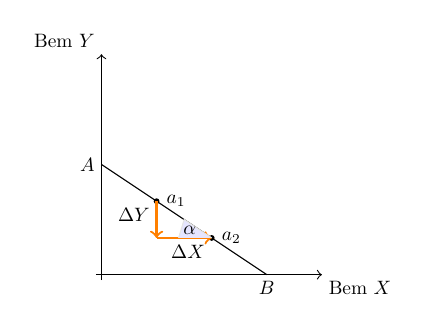
\begin{tikzpicture}[scale=0.7,every node/.style={scale=0.7}]
					\draw[->] (-0.1,0) -- (4,0) node[below right] {Bem $X$};
					\draw[->] (0,-0.1) -- (0,4) node[above left] {Bem $Y$};

					\draw[] (0,2) node[left] {$A$} -- (3,0) node[below] {$B$};

					\node[circle,fill=black,inner sep=0pt,minimum size=3pt,label=right:{$a_1$}] at (1,{4/3}) {};
					\node[circle,fill=black,inner sep=0pt,minimum size=3pt,label=right:{$a_2$}] at (2,{2/3}) {};

					\onslide<2->{
						\draw[orange,->,thick] (1,{4/3}) -- (1,{2/3});
						\node[below left] at (1,{4/3}) {$\Delta Y$};
					}

					\onslide<3->{
						\draw[orange,->,thick] (1,{2/3}) -- (2,{2/3});
						\node[below left] at (2,{2/3}) {$\Delta X$};
					}

					\onslide<4->{
						\draw[draw=black!10,fill=blue!10] (2,{2/3}) -- (1.5,1) -- (1.4,{2/3}); 
						\node[] at (1.6,.8) {$\alpha$};
					}

				\end{tikzpicture}
			\end{center}
		\end{column}
		
		\begin{column}{0.47\textwidth}
			\begin{itemize}
				\item \onslide<5->{$\left|\frac{\Delta Y}{\Delta X}\right|=|\tan{\alpha}|$, o que coincide com o declive da FPP linear (sem sinal) e designa-se custo relativo do bem $X$.}
				\item \onslide<6->{Representa um custo de oportunidade...}
			\end{itemize}
		\end{column}
	\end{columns}

\end{frame}

\begin{frame}
	\frametitle{Vantagens do Com\'ercio}

	\begin{itemize}
		\item H\'a ganhos que decorrem de os indiv\'iduos se especializarem nas tarefas que fazem melhor e recorrerem ao com\'ercio para trocarem entre si o produto das suas actividades \pause
		\item Usemos a FPP para tirar essa conclus\~ao
	\end{itemize}
\end{frame}

\begin{frame}
	\frametitle{Vantagens do Com\'ercio}
	Dois vizinhos, um sabe pintar e o outro sabe cozinhar... as suas FPP s\~ao descritas por:

	\vspace{0.1cm}

	\begin{columns}
		\begin{column}{0.47\textwidth}
			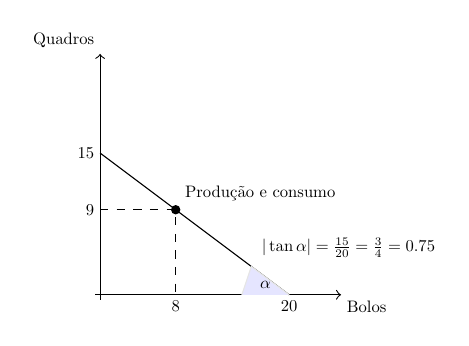
\begin{tikzpicture}[scale = 0.6, every node/.style={scale=0.6}]
				\draw[->] (-0.1,0) -- (5.1,0) node[below right] {Bolos};
				\draw[->] (0,-0.1) -- (0,5.1) node[above left] {Quadros};

				\draw[black] (0,3) node[left] {$15$} -- (4,0) node[below]{$20$};
				\draw[dashed] (0,1.8) node[left] {$9$} -- (1.6,1.8) node[circle,fill,inner sep=2pt,label=above right:Produ\c c\~ao e consumo]{} -- (1.6,0) node[below]{$8$};

				\draw[draw=black!10,fill=blue!10] (4,0) -- (3.2,.6) -- (3,0); 
				\node[] at (3.5,.2) {$\alpha$};

				\node[anchor = west] at (3.3,1) {$|\tan{\alpha}|=\frac{15}{20}=\frac{3}{4}=0.75$};
			\end{tikzpicture}
			\centering{\small{Pintor}}
		\end{column}
		\begin{column}{0.47\textwidth}
			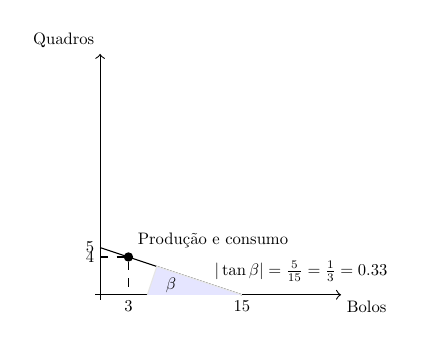
\begin{tikzpicture}[scale = 0.6, every node/.style={scale=0.6}]
				\draw[->] (-0.1,0) -- (5.1,0) node[below right] {Bolos};
				\draw[->] (0,-0.1) -- (0,5.1) node[above left] {Quadros};

				\draw[black] (0,1) node[left] {$5$} -- (3,0) node[below]{$15$};
				\draw[dashed] (0,0.8) node[left] {$4$} -- (0.6,0.8) node[circle,fill,inner sep=2pt,label=above right:Produ\c c\~ao e consumo]{} -- (0.6,0) node[below]{$3$};

				\draw[draw=black!10,fill=blue!10] (3,0) -- (1.2,.6) -- (1,0); 
				\node[] at (1.5,.2) {$\beta$};

				\node[anchor = west] at (2.3,0.5) {$|\tan{\beta}|=\frac{5}{15}=\frac{1}{3}=0.33$};
			\end{tikzpicture}
			\centering{\small{Cozinheiro}}
		\end{column}
	\end{columns}
\end{frame}

\begin{frame}
	\frametitle{Custos Relativos; Vantagem Comparativa}

	\begin{table}
		{\renewcommand{\arraystretch}{1.5}
		\begin{tabular}{cccc}
			Custos de Oportunidade & Pintor & & Cozinheiro \\
			\hline \hline
			Um bolo & $\frac{3}{4}$ & $>$ & $\frac{1}{3}$ \\
			Um quadro & $\frac{4}{3}$ & $<$ & $3$ \\
			\hline \hline
		\end{tabular}
		}
	\end{table}\pause
	\small{
	O cozinheiro tem vantagem comparativa na produ\c c\~ao de bolos, no entanto o pintor tem vantagem comparativa na produ\c c\~ao de quadros... \pause

	\vspace{0.2cm}

	Valer\'a a pena o pintor especializar-se na produ\c c\~ao de quadros se puder trocar cada um por mais do que $\frac{4}{3}$ de bolos (o custo de oportunidade)\pause

	\vspace{0.2cm}

	Valer\'a a pena o cozinheiro especializar-se na produ\c c\~ao de bolos, se puder trocar cada um por mais do que $\frac{1}{3}$ de quadro (ou seja, um quadro em troca de $3$ bolos no m\'aximo)	
	}
\end{frame}

\begin{frame}
	\frametitle{Termos de Troca}

	Estando o pintor disposto a receber $\frac{4}{3}$ de bolo por cada quadro que venda e estando o cozinheiro disposto a pagar $3$ bolos por cada quadro que compre, h\'a margem para transac\c c\~oes mutuamente vantajosas! \pause

	\vspace{0.2cm}

	Pode haver trocas se um quadro se trocar por um qualquer n\'umero de bolos entre $\frac{4}{3}$ e $3$.

\end{frame}

\begin{frame}
	\frametitle{Vantagens do com\'ercio}
	{\small Admitamos que h\'a especializa\c c\~ao e que o pintor vende $5$ quadros ao cozinheiro e que lhe compra $10$ bolos em troca... ent\~ao cada quadro trasaccionou-se em troca de $2$ bolos, o que \'e um valor interm\'edio entre o valor que o pintor estava disposto a receber para vender um quadro e o valor que o cozinheiro estava disposto a pagar.}
	
	\begin{table}
		\begin{adjustbox}{max width = \textwidth}
		{\renewcommand{\arraystretch}{1.5}
		\begin{tabular}{ccccccc}
			\multicolumn{2}{c}{} & \multicolumn{2}{c}{Autarcia} & \multicolumn{2}{c}{Com Com\'ercio} & \multirow{2}{*}{\parbox{2cm}{Ganhos de com\'ercio}}\\
			\cline{3-4}\cline{5-6} 
			\multicolumn{2}{c}{} & Produ\c c\~ao & Consumo & Produ\c c\~ao & Consumo & \\
			\hline\hline
			\multirow{2}{*}{Pintor} & Quadros & 9 & 9 & 15 & 10 & +1 \\
								    & Bolos   & 8 & 8 & 0  & 10 & +2 \\
			\hline
			\multirow{2}{*}{Cozinheiro} & Quadros & 4 & 4 & 0 & 5 & +1 \\
										& Bolos & 3 & 3 & 15 & 5 & +2 \\
			\hline\hline
		\end{tabular}
		}
		\end{adjustbox}
	\end{table}
\end{frame}

\begin{frame}
	\frametitle{Vantagens do Com\'ercio}
	Com com\'ercio, ambos os agentes econ\'omicos beneficiam, \\
	especializando-se no que fazem melhor (vantagem comparativa)

	\vspace{0.1cm}

	\begin{columns}
		\begin{column}{0.47\textwidth}
			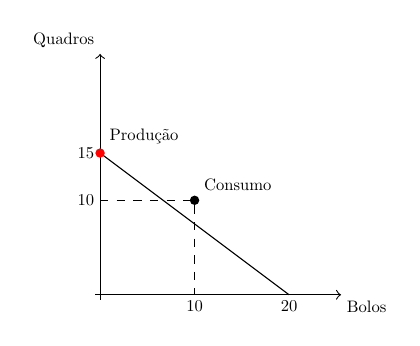
\begin{tikzpicture}[scale = 0.6, every node/.style={scale=0.6}]
				\draw[->] (-0.1,0) -- (5.1,0) node[below right] {Bolos};
				\draw[->] (0,-0.1) -- (0,5.1) node[above left] {Quadros};

				\draw[black] (0,3) node[left] {$15$} -- (4,0) node[below]{$20$};
				\draw[dashed] (0,2) node[left] {$10$} -- (2,2) node[circle,fill,inner sep=2pt,label=above right:Consumo]{} -- (2,0) node[below]{$10$};

				\draw (0,3) node[red,circle,fill,inner sep=2pt,label=above right:Produ\c c\~ao]{};
			\end{tikzpicture}
			\centering{\small{Pintor}}
		\end{column}
		\begin{column}{0.47\textwidth}
			\begin{tikzpicture}[scale = 0.6, every node/.style={scale=0.6}]
				\draw[->] (-0.1,0) -- (5.1,0) node[below right] {Bolos};
				\draw[->] (0,-0.1) -- (0,5.1) node[above left] {Quadros};

				\draw[black] (0,1) node[left] {$5$} -- (3,0) node[below]{$15$};
				\draw[dashed] (0,1) node[left] {$5$} -- (1,1) node[circle,fill,inner sep=2pt,label=above right:Consumo]{} -- (1,0) node[below]{$5$};

				\draw (3,0) node[red,circle,fill,inner sep=2pt,label=above right:Produ\c c\~ao]{};

			\end{tikzpicture}
			\centering{\small{Cozinheiro}}
		\end{column}
	\end{columns}
\end{frame}

\begin{frame}
	\frametitle{Vantagens do Com\'ercio}
	Possibilidades de Consumo se termos de troca forem 1 quadro trocado por 2 bolos...

	\vspace{0.1cm}

	\begin{columns}
		\begin{column}{0.47\textwidth}
			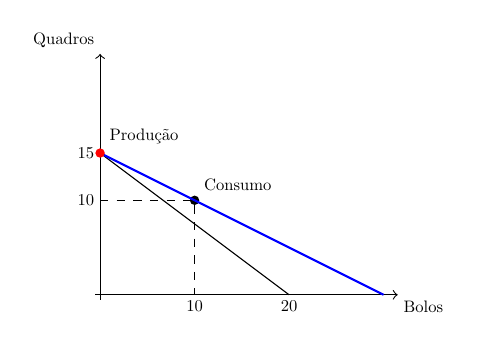
\begin{tikzpicture}[scale = 0.6, every node/.style={scale=0.6}]
				\draw[->] (-0.1,0) -- (6.3,0) node[below right] {Bolos};
				\draw[->] (0,-0.1) -- (0,5.1) node[above left] {Quadros};

				\draw[black] (0,3) node[left] {$15$} -- (4,0) node[below]{$20$};
				\draw[dashed] (0,2) node[left] {$10$} -- (2,2) node[circle,fill,inner sep=2pt,label=above right:Consumo]{} -- (2,0) node[below]{$10$};

				\draw[blue, thick] (0,3) -- (6,0);

				\draw (0,3) node[red,circle,fill,inner sep=2pt,label=above right:Produ\c c\~ao]{};
			\end{tikzpicture}
			\centering{\small{Pintor}}
		\end{column}
		\begin{column}{0.47\textwidth}
			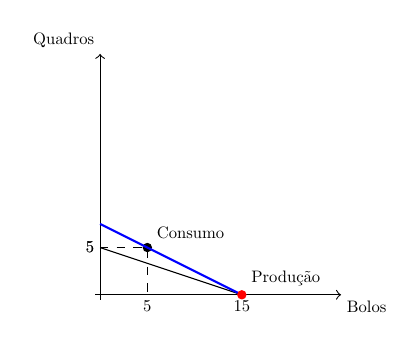
\begin{tikzpicture}[scale = 0.6, every node/.style={scale=0.6}]
				\draw[->] (-0.1,0) -- (5.1,0) node[below right] {Bolos};
				\draw[->] (0,-0.1) -- (0,5.1) node[above left] {Quadros};

				\draw[black] (0,1) node[left] {$5$} -- (3,0) node[below]{$15$};
				\draw[dashed] (0,1) node[left] {$5$} -- (1,1) node[circle,fill,inner sep=2pt,label=above right:Consumo]{} -- (1,0) node[below]{$5$};

				\draw[blue,thick] (0,1.5) -- (3,0);

				\draw (3,0) node[red,circle,fill,inner sep=2pt,label=above right:Produ\c c\~ao]{};

			\end{tikzpicture}
			\centering{\small{Cozinheiro}}
		\end{column}
	\end{columns}
\end{frame}

\begin{frame}
	\frametitle{Vantagem comparativa}
	\begin{itemize}
		\item No exemplo, o pintor tem vantagem comparativa na produ\c c\~ao de quadros porque o seu custo de oportunidade \'e menor do que o do cozinheiro: precisa de prescindir de menor quantidade de produ\c c\~ao de bolos para utilizar o seu tempo na produ\c c\~ao de quadros do que o cozinheiro precisaria se quisesse produzir mais um quadro...

		\item \'E da vantagem comparativa que dependem os ganhos do com\'ercio e os padr\~oes de especializa\c c\~ao
	\end{itemize}
\end{frame}

\begin{frame}
	\frametitle{Vantagem comparativa}
	\begin{itemize}
		\item O com\'ercio (neste caso, troca directa) tem a vantagem de permitir que cada um dos agentes econ\'omicos se especialize na tarfe que faz relativemnte melhor, para que depois eles se encontrem no mercado para fazerem transac\c c\~oes.
		\item Ap\'os o com\'ercio, \'e poss\'ivel os indiv\'iduos estarem num ponto de consumo em que obt\^em mais quantidade de ambos os bens, do que numa situa\c c\~ao de autarcia, usando so mesmos recursos.

		\item Todos temos uma vantagem comparativa nalguna actividade... o mesmo se aplica a empresas, a pa\'ises... \'e neste princ\'ipio que se baseia o com\'ercio internacional.
	\end{itemize}
\end{frame}